\subsection{Preguntas}	
	\begin{enumerate}
		\item ¿Cuál es la diferencia entre un Switch y un router? ¿Qué tienen en común?
		\item ¿Cuál es la diferencia entre un Switch convencional y un Switch OpenFlow?
		\item ¿Se pueden reemplazar todos los routers de la Intenet por Swithces OpenFlow?\\
		Piense en el escenario interASes para elaborar su respuesta
	\end{enumerate}

\subsection{Maquina virtual}
	Necesitamos de la maquina virtual (VM) para poder ejecutar el controlador, el firewall y la topologia. Por lo tanto debemos usar 		distintas terminales de la misma oara ello. Hay dos formas de hacer esto, una es usar la interfaz que provee la VM y abrir terminales 		desde alli. La otra es abrir terminales desde nuestra pc, y conectarnos via ssh a la maquina virtual. Parece que la primera opcion es 		mas comoda, pero en mi experiencia la VM se traba mucho mas.
	Para conectarse via ssh a la VM, primero clonamos nuestro repositorio y solo necesitamos ejecutar un script que hace el trabajo.
	\begin{lstlisting}[language=bash]
		sh scripts/conect_to_VM.sh
	\end{lstlisting}
	Nos pedira la cotraseña de nuetra pc, y luego la contraseña de la VM que es: $frenetic$.\\
	Luego, si queremos tener nuestro repositorio en la VM, y ademas el controlador en la carpeta $pox/ext$ del repositorio de pox en la VM, 	debemos ejecutar el siguiente comando:\\
	\begin{lstlisting}[language=bash]
		sh scripts/resync.sh
	\end{lstlisting}
\subsection{Topologia}
	La topologia que se desarrollo se llama Fat tree. En la figura 5 vemos nuetra topologia por defecto que es un árbol de altura 3.
	La raiz tiene conectada 3 hosts que funcionan como clientes del datacenter, cada una de las raices a su vez, tendrán conectadas un host 	cada una, que funcionará como proveedor de contenido.\\
	Los tres hosts clientes se comunican con los hosts del datacenter usando los protocolos ICMP, TCP y UDP.
	\begin{figure}[ht]
		\begin{adjustbox}{addcode={
			\begin{minipage}{\width}}{
				\caption{%
					Ejemplo de como seria la topologia con un arbol de altura 3.
					}
			\end{minipage}},rotate=360,center}
			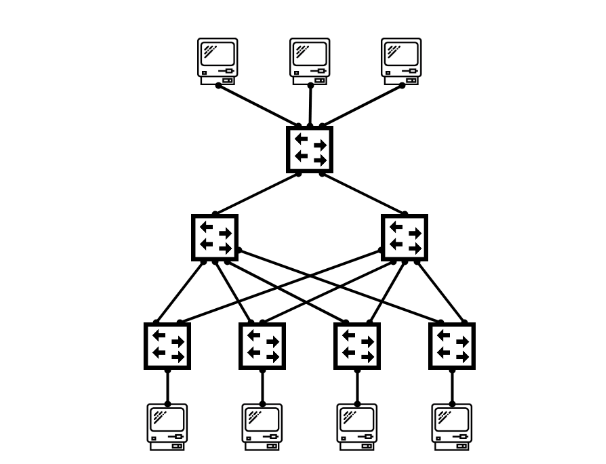
\includegraphics[scale=.6]{pics/topologia-arbol-altura-3.png}
		\end{adjustbox}
	\end{figure}
	\FloatBarrier
	Para poder levantar la topologia sin pasarle los argumentos de configuracion, lo cual hace que por defecto tenga tres clientes y una 		altura de tres, abrimos una terminal que este en la raiz del sistema de archivos de la maquina virtual y podemos escribir 
	lo siguiente:\\
	\begin{lstlisting}[language=bash]
		sudo mn --custom ~/Datacenter/src/topology.py --topo mytopo --mac --switch ovsk --controller remote
	\end{lstlisting}
	En caso de querer configurar la altura o cantidad de clientes, podemos escribir lo siguiente:\\
	\begin{lstlisting}[language=bash]
		sudo mn --custom ~/Datacenter/src/topology.py --topo mytopo, levels=4, clients=4 --mac --switch ovsk --controller remote
	\end{lstlisting}

\subsection{Controlador}
	El controlador se encarga de la logica del balanceo de cargas y tambien se encarga de llenar las tablas de los switch cuando estos les 		llega un mensaje que no saben responder. De esta manera nuestro controlador consta de $handlers$ los cuales se ejecutan cuando un 		switch acude al controlador.\\
	El controlador hace un estudio de la topologia para poder obtener un diccionario de adyacencias, el cual sera util para poder calcular 		el camino minimo para el balanceo de cargas.\\
	\underline{\textbf{\_handle\_LinkEvent:}}\\
		Este handler es invocado cada vez que se detecta un link entre switches. El modulo $Discovery$ es el que se encarga de esto. Se 		envias mensajes LLDP entre los switches y estos mismos responden, y de esta manera se puede aprender la topologia. En nuestro 			handler, cuando es invocado, llenamos un diccionario con la informacion pertinente.\\
	\underline{\textbf{host\_tracker:}}\\
		Es una clase de python que se encuantra en el repositorio de pox. En nuestro caso la utilizamos para poder descubrir el 		identificador del switch destino a partir de la direccion mac destino. Esto lo necesitamos porque las adyacencias se manejan 			con los identificadores de los switchs (dpid). Por eso, en el constructor del controlador se instancia el mismo, y por cada vez 		que se entra al handler que se encarga de llenar la tabla de los switches ($\_handle\_PacketIn$), se llama al handler del 			$host\_tracker$, que se encarga de aprender los dpid. Luego, podremos obtener el identificador utilizando un metodo del 		$host\_tracker$ el cual accede a un diccionario de entradas de direcciones mac, y retorna el dpid. 
		Ese metodo es $host\_tracker.getMacEntry(addr)$\\
	\underline{\textbf{spanning tree:}}\\
		Este modulo se encarga de eliminar los ciclos de la topologia. Su función es la de gestionar la presencia de bucles en 			topologías de red debido a la existencia de enlaces redundantes. El protocolo permite a los dispositivos de interconexión 			activar o desactivar automáticamente los enlaces de conexión, de forma que se garantice la eliminación de bucles.\\
	\underline{\textbf{\_handle\_PacketIn:}}\\
		Este handler se invoca frente a la llegada de un paquete, cuando un switch no sabe como responder frente a el, es decir, la 			tabla del switch no tiene un $match$ para despacharlo por un puerto, por lo tanto, le pide ayuda al controlador. El algoritmo 			es bastante simple y consta de los siguientes pasos:
		\begin{itemize}
			\item Se llama al handler del $host\_tracker$ para que aprenda los dpid de cada mac.
			\item Si la topologia aun no fue aprendida, se retorna.
			\item Si el protocolo no es ni ICMP, o TCP o UDP se retorna
			\item Si el paquete es IPv6 se retorna
			\item Si el paquete ethernet no se encuentra, se retorna
			\item Si el paquete no es ni IP ni ARP, se retorna.
			\item Si la direccion mac destino, no se encuantra en nuestra tabla de matcheo de mac con dpid (generada a partir de la 			respuesta del $host\_tracker$ al invocar $host\_tracker.getMacEntry(addr)$) se hace flooding y retorna
			\item Si el dpid origen coindide con el destino, no hacemos nada y guardamos esto en la tabla.
			\item si son distintos:
			\begin{itemize}
				\item Se buscan todos los caminos minimos desde el dpid origen al destino en el diccionario de adyacencias.
				\item Si no hay caminos, se retorna
				\item si, existen caminos, se extrae de ellos los puertos de los cuales se sale del switch (seria el puerto de 					salida)
				\item Se actualiza la tabla del switch
				\item se envia el mensaje.
			\end{itemize}
		\end{itemize}
	\underline{\textbf{Tecnica ECMP - Balanceo de cargas:}}\\
		Para resolverlo se creo una clase en python llamada $ECMPTable$ la cual encapsula un diccionario que tiene como clave el 			identificador del switch corresponiente ($dpid$). Como valor de este identificador tiene otro diccionario en el cual su clave 			se una tupla de valores los cuales son, el identificador del switch destino ($dst\_dpid$), la direccion mac origen 
		($src\_addr$), la direccion mac destino ($dst\_addr$), y un string que nos dice el protocolo ($protocol$: [ICMP, TCP, UDP]). 			Como valor a esta clave se encuentra el puerto de salida. De esta manera, frente a distintos caminos de igual peso, dependiendo 		el flujo, los puertos de salida son distintos.

\subsection{Firewall}
	Se creo una clase llamada Firewall la cual, frente a la llegada de paquetes UDP, en caso de superar cierto maximo (en nuestro caso 		100), se los bloquea. Luego de un tiempo, se los desbloquea. Para poder llevarlo a cabo, se creo un metodo 
	llamado	$request\_for\_switch\_statistics$, el cual se llama cada un tiempo determinado mediante un timer. Este se encarga de pedirle 		las estadisticas a los switches, para poder calcular la frecuencia de paquetes UDP. Luego, tenemos otro handler 
	llamado $\_handle\_flowstats\_received$ el cual se llama cada vez que los witches nos proveen sus estadisticas. El algoritmos se 		pregunta que los paquetes tengan el protocolo UDP, y almacena su cantidad en un diccioanrio. En caso de que la diferencia de cantidades 	entre la vez actual y la anterior acumulada sea mayor que nuestro maximo propuesto, se procede a bloquear el paquete y se setea un 		timer para este. En caso de no superar est maximo, se chequea si ya se esta bloqueado, y en ese caso se chequea el paso del tiempo con 		los timers.

\subsection{Launch}
	Para poder levantar el controlador y el firewall, se creo un archivo llamado $launch.py$ que configura el spanning tree, el discovery, 		el controlador y el firewall.






